\subsection{Energieversorgung}
\label{subsec:Energieversorgung}
Die verschiedenen Bauteile auf dem PCB müssen mit Energie versorgt werden. Gemäss Auftragsbeschreibung soll die Wetterstation desweiteren über Photovoltaik gespiesen werden. Da die Sonne nur tagsüber scheint und um eine konstante Versorgung gewährleisten zu können, wird ein Akku benötigt. Um die Speisung via Akku und gleichzeitig ein Speisen des Akkus über die Photovoltaikanlage zu gewährleisten, muss der Ladestrom geregelt werden, was mit einem Power-Management-IC, dem MCP73871, erfolgt. Der MCP73871 führt die Speisung des Akkus weiter auf einen Linearregler (LM1117), welcher das 3.3V-Netz generiert. Damit der LM1117 eine saubere Ausgangsspannung (3.3V mit möglichst kleinem Rippel) generieren kann, muss dieser einen erhöhten Spannungspegel am Eingang haben, weshalb eine ChargePump (Ladungspumpe) benötigt wird. Das Konzept der Energieversorgung wird in Kapitel \ref{sec:Konzept} vorgestellt, weshalb nun die Berechnung der Akkukapazität, der Einfluss der Photovoltaik, sowie die Kombination von ChargePump und Linearregler näher erläutert werden.
%\subsubsection{Energiekonzept}
%\label{subsubsec:Energiekonzept}
%In diesem Kapitel wird das Energiekonzept erläutert. Dies soll eine Übersicht über die Energieversorgung geben.\\
%\begin{figure}[hbtp]
%\centering
%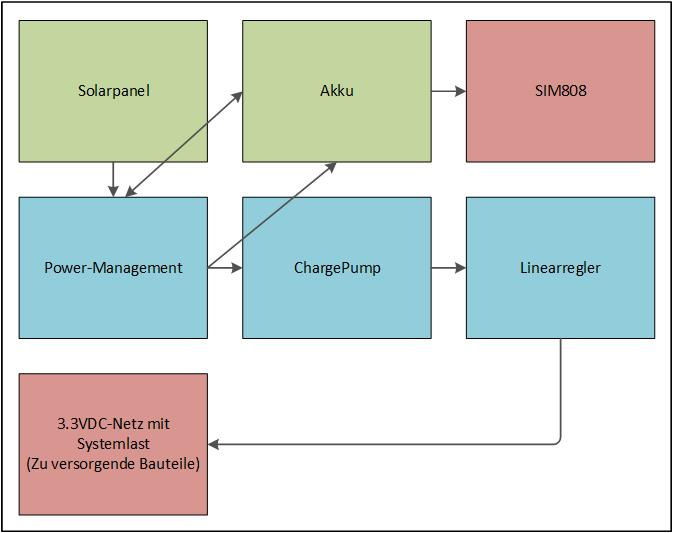
\includegraphics[width=0.8\textwidth]{graphics/Energieversorgung/Konzept.JPG}
%\captionof{figure}{Konzept der Energieversorgung}
%\label{fig:Energiekonzept}
%\end{figure}\\
%\newpage
%Abbildung \ref{fig:Energiekonzept} zeigt das Konzept der Energieversorgung. Darin sind Grün markiert die Energielieferanten, Blau die Schaltung um das 3.3V-Netz zu generieren und Rot die Verbraucher. Das Solarpanel speist über das Power-Management (MCP73871) den Akku. Der Akku ist die Quelle für die gesamte Wetterstation und speist diese ebenso über den MCP73871. Die Spannung des Akkus wird über den MCP73871 auf die ChargePump gegeben und dort erhöht, so dass der nachfolgende Linearregler (LM1117) mit dieser erhöhten Spannung einen möglichst konstanten (rippelfreien) 3.3V-Ausgang generiert. Mit diesem Ausgang des LM1117 wird das 3.3V-Netz generiert, woraus die benutzten Bauteile (die Systemlast) ihre benötigte Spannung erhalten. Einzige Ausnahme bildet hier der SIM808, da dieser eine höhere Spannung benötigt. Da der SIM808 eine erhöhte Betriebsspannung hat und Stromspitzen für das Senden und Empfangen von SMS aufweist, wird dieser direkt über den Akku betrieben. Falls die Wetterstation nicht benötigt werden sollte, können die Verbraucher über ein Schalter abgeschaltet werden. Es ist zu beachten, dass das Benutzen des Schalters die Energieversorgung sofort komplett trennt und auf dem PCB diverse Kondensatoren vorhanden sind, welche sich noch entladen. Ausserdem wird der MCP73871 nicht ausgeschaltet, weshalb ein weiteres laden des Akkus über die Photovoltaik möglich ist.
\subsubsection{Berechnung der Akkukapazität}
Um die Kapazität des Akkus zu berechnen, muss eine Schätzung des Energieverbrauchs gemacht werden. In Tabelle \ref{tab:Energieverbrauch} werden deshalb die verwendeten Bauteile mit ihrem Stromverbrauch aufgelistet.
\begin{table}[h]
	\centering
	\caption{Übersicht über die verwendeten Bauteile mit ihrem Stromverbrauch.}
	\small
  \begin{tabular}{lllllll}
  \toprule 
  \textbf{Bauteilname} & \textbf{Modus} & \textbf{Min} & \textbf{Typ} & \textbf{Max} & \textbf{Einheit}\\ 
  \midrule 
  MCP73871 \cite{MCP73871}& Charge Complete &  & 120 & 200 & $\mu$A  \\ 
  \hline 
  LM1117 \cite{LM1117} &  & & 5 & 10 & mA   \\ 
  \hline 
  SIM808 \cite{SIM808}& PWR Down &  & 38 & 50 & $\mu$A   \\ 
   & Idle  &  & 22.1 &  & mA  \\ 
   & Data GSM &  & 445.82 &  & mA   \\ 
   & GPS acquisition &  & 42 &  & mA   \\ 
   & GPS continuous tracking &  & 24 &  & mA   \\ 
   & TX Burst (peak)  &  & 2 &  & A  \\ 
  \hline 
  Anemometer &  &  &  &  &   \\ 
  \hline 
  Ombrometer &  &  &  &  &   \\ 
  \hline 
  Windrichtungsgeber \cite{ADSkeineAngabe}&  & 0.028 &  & 4.8 & mA \\ 
  \hline 
  74VHC125 \cite{74HC125}&  & 20 &  & 40 & $\mu$A  \\ 
  \hline 
  ATMega2560 \cite{arduinoMega}& active &  & 7 &  & mA  \\ 
  \hline
  PN2222A & active &  & 600 &  & mA  \\
  \hline 
  FT231XS \cite{FTDI}& normal & 8 & 8 & 8.4 & mA \\ 
   & USB suspend &  & 125 &  & $\mu$A \\ 
  \hline 
  74HC4050 \cite{74HC4050}&  &  &  & 40 & $\mu$A \\ 
  \hline 
  BME280 \cite{Bosch2019}& standby &  & 0.2 & 0.5 & $\mu$A  \\ 
   & humidity measuring &  & 340 &  & $\mu$A \\ 
   & pressure measuring &  & 714 &  & $\mu$A  \\ 
   & temperature measuring &  & 350 &  & $\mu$A \\ 
  \hline 
  TSL2561 \cite{TSL2561}& active &  & 0.24 & 0.6 & mA \\ 
   & power down &  & 3.2 & 15 & $\mu$A  \\ 
  \hline 
  DS3231 \cite{DS3231DS}& active & &  & 200 & $\mu$A \\ 
   & standby &  & & 110 & $\mu$A  \\ 
  \bottomrule 
  \end{tabular} 
	\label{tab:Energieverbrauch} 
\end{table}
\newpage
Tabelle \ref{tab:Energieverbrauch} zeigt den Stromverbrauch der verwendeten Bauteile gemäss ihren Datenblättern. Das Anemometer und das Ombrometer besitzen keine Werte, da nur beim Schliessen eines der integrierten Reedkontakte ein Strom fliesst, weshalb diese Ströme vernachlässigt werden. Die Ströme des Windrichtungsgebers wurden berechnet anhand der 3.3V Versorgungsspannung und den Widerstandswerten gemäss Datenblatt. Vom MCP73871 wurde lediglich der Strom bei geladenem Akku genommen, da das Laden des Akkus mit dem Ladestrom der Photovoltaik erfolgt und somit nicht direkt ein Verbrauch ist. Der SIM808 besitzt mit seinen 2A Spitzenstrom bei einem TX Burst (senden einer SMS) den höchsten Konsum, jedoch ist dieser Burst lediglich 577$\mu$s lang und wird somit auch nicht berücksichtig, zumal nicht gesagt werden kann wie oft dieser Burst tatsächlich vorkommt. Der SIM808 wird im Normalbetrieb das GPS im continuous tracking und das GSM im Idle Modus haben, weshalb hier insgesamt ein Strom von Typ 46,1 mA verbraucht wird. Der ATMega2560 wird im Normalbetrieb stets im active Modus sein, weshalb nur dieser Wert aus dem Datenblatt ausgelesen wurde. Die serielle Schnittstelle wird im Normalbetrieb nicht benutzt (kein Notebook angehängt), weshalb beim FT231XS der USB suspend Modus zur Berechnung benutzt und der PN2222A vernachlässigt wird. Der BME280 sollte stets Messungen durchführen, weshalb hier mit dem höchsten Wert (pressure measuring Modus) gerechnet wird. Ähnlich verhält es sich beim TSL2561 und beim DS3231, hier werden die active Modi in die Rechnung mit einbezogen.\\[0.5cm]
Um den SIM808 mit einer optimalen Spannung versorgen zu können, wird ein Akku mit einer Spannung von 4V benötigt. Der Gesamtstrombedarf im Normalbetrieb beläuft sich gemäss Tabelle \ref{tab:Energieverbrauch} und verwendeten Maximalwerten auf rund 70mA. Multipliziert man die Spannung mit dem Gesamtstrombedarf, so ergibt dies eine Leistung von 0.28 Watt. Um daraus die benötigte Akkukapazität zu ermitteln, muss festgelegt werden, wie lange dieser die Wetterstation mindestens speisen können soll. Gemäss Pflichtenheft soll der Akku die Wetterstation für mindestens 100 Stunden aufrecht erhalten können. Die berechnete Leistung wird mit den Anzahl Stunden multipliziert, was 28 Wh ergibt. Bei einer Akkuspannung von 4V ergibt das (durch dividieren der 28 Wh mit den 4V) eine Mindest-Akkukapazität von 7Ah oder auch 7000mAh.
\subsubsection{Einfluss der Photovoltaik}
Die Photovoltaik (das Solarpanel) erzeugt Strom durch Sonnenenergie. Der erzeugte Strom wird dazu verwendet den Akku zu laden, während dieser die Wetterstation speist. Im vorhergehenden Kapitel wurde die benötigte Leistung der Wetterstation von 0.28 Watt berechnet und die daraus Resultierende Mindest-Akkukapazität von 7000mAh. Gemäss Pflichtenheft soll das Solarpanel den Akku innert einem Tag laden können.\\

\begin{figure}[h]
\centering
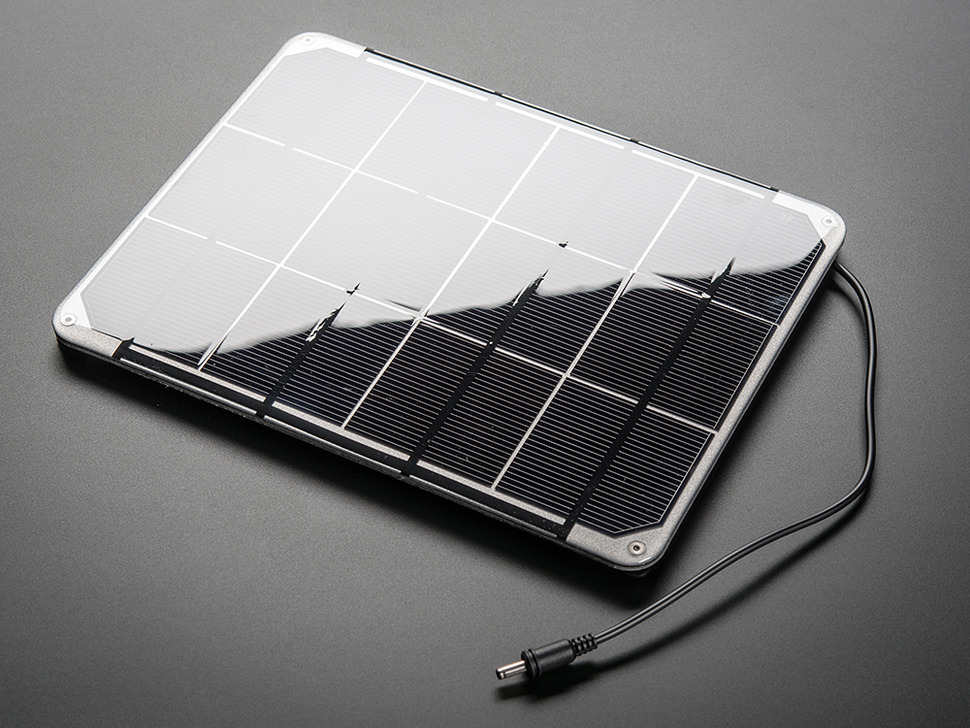
\includegraphics[width=0.4\textwidth]{graphics/Energieversorgung/Solarpanel.JPG}
\captionof{figure}{6V 6W Solarpanel von Adafruit \cite{Solarpanel}}
\label{fig:Solarpanel}
\end{figure}
\newpage
Da das Solarpanel nur bei Sonneneinstrahlung Strom erzeugen kann und die Sonnenstunden von Land zu Land abweichen, werden bei dieser Rechnung 6 Sonnenstunden pro Tag angenommen. Um 7000mAh innert 6h laden zu können, müssen konstant 1166.66mA bzw. rund 1.2A Strom erzeugt werden. Hier beschränkt jedoch der MCP73871, da dieser bei dementsprechender Beschaltung ein Fast Charge Current von Typ 1A und Max 1.1A zulässt. Rechnet man zurück so wird das Solarpanel typischerweise 7h benötigen um bei einem erzeugten Ladestrom von 1A den Akku voll zu laden. Während den Sommermonaten sollte dies in den meisten Gegenden kein Problem darstellen, doch könnte dies über die Wintermonate nicht reichen. Um dies zu verifizieren rechnen wir den Verbrauch der Schaltung pro Tag aus und schauen, wie viele Sonnenstunden das Solarpanel bräuchte um bei 1A Ladestrom den Verbrauch auszugleichen. Bei 0.28W Verbrauch und 24h pro Tag ergibt das 6.72Wh. Da der Akku 4V liefert folgen daraus 1.68Ah Verbrauch für den Akku. Geht man wieder von einem Ladestrom von 1A aus, so werden 1.68 Sonnenstunden benötigt bei denen das Solarpanel 1A Ladestrom erzeugt um den Verbrauch zu decken. Aus diesem Grund kann gesagt werden, dass jedes Solarpanel wegen des MCP73871 nicht ausreichen wird, um die Mindest-Akkukapazität von 7000mAh innert 6 Sonnenstunden laden zu können. Wird jedoch ein Solarpanel verwendet das 1A Ladestrom erzeugen kann, so werden lediglich 1.68 Sonnenstunden benötigt um den Verbrauch zu decken. Für die Wetterstation wurde ein 6V 6W Solarpanel von Adafruit implementiert (Abbildung \ref{fig:Solarpanel}, was somit 1A Ladestrom erzeugen kann und ausreicht um den Verbrauch der Wetterstation innert 1.68 Sonnenstunden zu decken \cite{Solarpanel}.\\

\subsubsection{ChargePump und Linearregler}
Die Wetterstation besteht aus einigen Bauteilen, welche eine 3.3V-Versorgungsspannung benötigen. Da der Akku eine höhere Spannung liefert, muss ein Linearregler die Spannung auf 3.3V regeln. Dafür wird der LM1117 verwendet, welcher eine Eingangsspannung von bis zu Max 15V aushält. Damit der LM1117 die Eingangsspannung sauber (möglichst ohne Rauschen) auf die 3.3V regeln kann, sollte die Eingangsspannung mindestens 5V betragen. Um von den 4V Batteriespannung auf mindestens 5V zu gelangen, wird eine ChargePump verwendet. Eine ChargePump ist eine Schaltung, welche aus einem Schalter, 2 Kondensatoren und 2 Dioden besteht, wie in Abbildung \ref{fig:ChargePump} schematisch dargestellt. 

\begin{figure}[h]
\centering
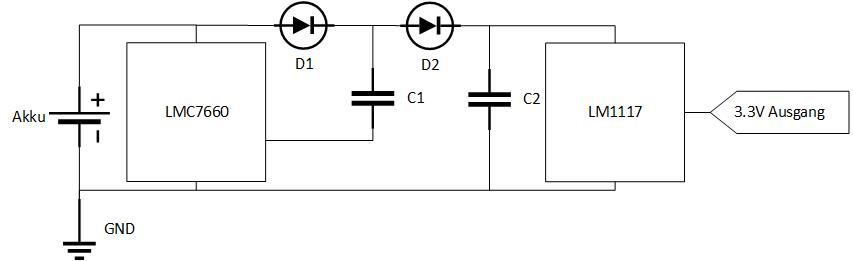
\includegraphics[width=1\textwidth]{graphics/Energieversorgung/ChargePump.JPG}
\captionof{figure}{Schematische Darstellung der ChargePump.}
\label{fig:ChargePump}
\end{figure}
\newpage
Abbildung \ref{fig:ChargePump} zeigt die Schematische Darstellung der verwendeten ChargePump. Als Schalter wird der LMC7660 verwendet, welcher zwischen 2 Stromkreisen wechselt. Das wechseln der Stromkreise bewirkt das aufladen des jeweiligen Kondensators. Im ersten Schalterzustand bilden D1, C1 und der Akku einen Stromkreis, wobei sich C1 auf die Akkuspannung lädt (abzüglich der Diodenspannung von D1). Im zweiten Zustand ist der Akku in Serie zu C1, welcher nun als Spannungsquelle fungiert, und der Kondensator wird auf die doppelte Akkuspannung (abzüglich der Diodenspannungen) geladen. In beiden Zuständen sorgen die Dioden dafür, dass sich der Kondensator kontrolliert auf die gewünschte Seite hin entlädt. Durch diese ChargePump soll im Idealfall eine Spannung von etwa 6.6V (Doppelte Akkuspannung von 8V abzüglich der zwei Diodenspannungen von je ca. 0.7V) generiert werden können. Durch diese erhöhte Spannung ist es dem LM1117 möglich die Spannung auf 3.3V zu regeln, wobei durch Toleranzen ein nur relativ kleiner Rippel entsteht. Die Spannung am Ausgang des Linearreglers ist Ausgangspunkt für die Speisespannungen der Bauteile, welche eine 3.3V-Speisespannung benötigen.\\[0.5cm]
Nun wurde die Energieversorgung ebenfalls detailiert erläutert. Auf die verschiedenen Bauteilgruppen wurden nun in den verschiedenen Kapiteln jeweils näher eingegangen. Im nächsten Kapitel wird deshalb die Realisierung der Wetterstation auf einem PCB (Printed Circuit Board) thematisiert.
